%template1.tex
%The following LaTeX source file represents the simplest kind of slide presentation; no overlays, no included graphics. Substitute your favorite style for ``pascal''. To create the PDF file template1.pdf, (1) be sure to use the prosper class, then (2) execute the command latex template1.tex, and (3) the command dvipdf template1.dvi.

%%%%%%%%%%%%%%%%%%%%%%%%%%%%%%% template1.tex %%%%%%%%%%%%%%%%%%%%%%%%%%%%%%%%%%%
\documentclass[a4paper,blends,pdf,colorBG,slideColor]{prosper}
% definitions for slides for CSC544
% Lutz Hamel, (c) 2007

\hypersetup{pdfpagemode=FullScreen}

\usepackage{amssymb}
\usepackage{latexsym}
\usepackage{amsmath}
%\usepackage[usenames]{color}
\usepackage{xypic}


\newcommand{\term}[1]{\ensuremath{\mbox{\bf #1}}}
\newcommand{\nonterm}[1]{\ensuremath{\mbox{#1}}}
\newcommand{\ifstmt}[3]{\ensuremath{{\bf if}\; {#1}\;{\bf then}\;{#2}\;{\bf else}\;{#3}\;\term{end}}}
\newcommand{\whilestmt}[2]{\ensuremath{{\bf while}\; {#1}\;{\bf do}\;{#2}\; \term{end}}}
\newcommand{\funcstmt}[3]{\ensuremath{{\bf fun}\; {#1}\; {\bf is}\; {#2} \; {\bf return}\; {#3}}}
\newcommand{\syntaxset}[1]{\ensuremath{\mbox{\bf #1}}}
\newcommand{\orbar}{\;|\;}
\newcommand{\bs}[1]{\begin{slide}{#1}\ptsize{8}}
\newcommand{\es}{\end{slide}}
\newcommand{\co}{\,\colon\;}
\newcommand{\pair}[2]{\ensuremath{\langle {#1}, {#2} \rangle}}
\newcommand{\encode}[1]{\ensuremath{\langle {#1} \rangle}}
\newcommand{\mytab}{\makebox[.15in]{}}
%\newcommand{\abs}[1]{{\mid{#1}\mid}}
\newcommand{\abs}[1]{{|{#1}|}}
\newcommand{\ol}[1]{\overline{#1}}

\newcommand{\qaccept}{\ensuremath{q_{\mbox{\tiny accept}}}}
\newcommand{\qreject}{\ensuremath{q_{\mbox{\tiny reject}}}}
\newcommand{\accept}{{\em accept}}
\newcommand{\reject}{{\em reject}}

\newcommand{\machine}[1]{
	\begin{quote}
	{#1}
	\end{quote}
	}

\newcommand{\fdef}[1]{
	\begin{center}
	\fbox{
	\begin{minipage}{3.5in}
	{\bf Definition:}
	{#1}
	\end{minipage}
	}
	\end{center}
	}

\newcommand{\ftheorem}[1]{
	\begin{center}
	\fbox{
	\begin{minipage}{3.5in}
	{\bf Theorem:}
	{#1}
	\end{minipage}
	}
	\end{center}
	}

\newcommand{\flemma}[1]{
	\begin{center}
	\fbox{
	\begin{minipage}{3.5in}
	{\bf Lemma:}
	{#1}
	\end{minipage}
	}
	\end{center}
	}


\newcommand{\fframe}[1]{
	\begin{center}
	\fbox{
	\begin{minipage}{3.5in}
	{#1}
	\end{minipage}
	}
	\end{center}
	}

\newcommand{\nframe}[1]{
	\begin{center}
	\begin{minipage}{3.5in}
	{#1}
	\end{minipage}
	\end{center}
	}

\begin{document}

\bs{Cook-Levin Theorem}
In the 1970's Stephen Cook and Leonid Levin independently discovered that there
are problems in $NP$ whose complexity are related to all other problems in $NP$ -- these problems are called $NP$-complete problems.

As we have seen, $NP$-complete problems are related to other $NP$ problems 
via polynomial reductions.

The first and most famous $NP$-complete problem discovered was a problem 
around the satisfiability of logic formulas.


\es

\bs{$SAT$}
{\small
A Boolean formula is an expression involving Boolean variables ($x$, $y$, {\em etc.}) and operations ($\wedge$, $\vee$, $\neg$, where $\neg x = \overline{x}$), 
\[
\phi = (\overline{x} \wedge y) \vee (x \wedge \overline{z}).
\]

A Boolean formula is satisfiable if some assignment of $true$ and $false$ to the variables of the formula makes the formula evaluate to $true$.

For example, the assignment
\[
\begin{array}{l}
x = false\\
y = true\\
z = false
\end{array}
\]
will make $\phi$ above evaluate to true.

The {\bf\em satisfiability problem} is to test whether a Boolean formula is satisfiable,
that is
\[
SAT = \{ \encode{\phi}| \mbox{$\phi$ is a satisfiable Boolean formula}\}.
\]
}
\es

\bs{$SAT$}
{\small
\ftheorem{{\bf (Cook-Levin)} 
\[
SAT \in \mbox{$NP$-complete}.
\]
}
{\bf Proof Sketch:}  For an $NP$-complete problem we need to show that it is in 
$NP$ and that all $A \in NP$ reduce to it.

(a)  It is easy to see that a truth assignment to the variables of a formula can be
checked in polynomial time.

(b) We need to show that $A \le_p SAT$ for all $A \in NP$.  This is done by
simulating the computations of a NTM deciding $A$ on some string $w$ using
Boolean formulas such that
\[
w \in A \mbox{ iff } f(w) \in SAT
\]
where $f$ converts the string $w$ into the Boolean formula $f(w)$.\footnote{For details, please see the Cook-Levin Theorem in the book.}$\Box$

{\bf Note:} In some sense this reinforces our notion that first-order logic is a powerful
language to reason about complex problems.
}
\es

\bs{$3SAT$}
{\small
The $3SAT$ problem:
\begin{itemize}
\item A special case of $SAT$,
\item Formulas are in {\em conjunctive normal form} (cnf),
\[
\underbrace{(x_1 \vee \overline{x_2} \vee \overline{x_3} \vee x_4)}_{\mbox{\scriptsize clause}} \overbrace{\wedge}^{\mbox{\scriptsize conjunction}} (x_3  \vee \overline{x_5} \vee x_6)\wedge(x_3 \vee \overline{x_6}),
\]
\item 3cnf -- each clause in the cnf has only 3 literals (or variables),
\[
(x_1 \vee \overline{x_2} \vee \overline{x_3}) \wedge (x_3 \vee \overline{x_5} \vee x_6),
\]
\end{itemize}

We define,
\[
3SAT = \{ \encode{\phi} | \mbox{$\phi$  is a satisfiable 3cnf formula}\}.
\]

}
\es

\bs{$3SAT$}
{\small
\ftheorem{
\[
3SAT \in \mbox{$NP$-complete}.
\]
}

{\bf Proof Sketch:} We show this by constructing a polynomial time reduction from $SAT$
to $3SAT$.

First, observe that any formula $\phi \in SAT$ can be rewritten in cnf such that
$\hat{\phi} = c_1 \wedge c_2 \wedge \ldots \wedge c_m$ where each clause $c_i$ is a
disjunction of Boolean variables, say $z_1 \ldots z_n$.

We now construct the polynomial time reduction $f\co SAT \rightarrow 3SAT$ such
$f(\hat{\phi}) = \phi_{3SAT}$.  We replace each $c_i$ in $\hat{\phi}$ by a collection
of literal clauses over the variables which appear in $c_i$ plus some additional variables which appear only in these 3 literal clauses.  More specifically, let $c_i = z_1 \vee z_2 \vee \ldots \vee z_k$ where each $z_j$ is a Boolean variable, then
\begin{description}
\item[$k = 1$:] Here $c_i = z_1$.  Use the additional variables $y_{i,1}$ and $y_{i,2}$
to construct the clauses in 3cnf
\[
(z_1\vee y_{i,1}\vee y_{i,2}) \wedge (z_1\vee \ol{y_{i,1}}\vee y_{i,2}) \wedge (z_1\vee y_{i,1}\vee \ol{y_{i,2}}) \wedge (z_1\vee \ol{y_{i,1}}\vee \ol{y_{i,2}})
\]
\item[$k=2$:] Here $c_i = (z_1 \vee z_2)$.  Use the additional variable $y_{i,1}$ to
construct the clauses in 3cnf
\[
(z_1 \vee z_2 \vee y_{i,1}) \wedge (z_1 \vee z_2 \vee \ol{y_{i,1}}) 
\]
\item[$k = 3$:] Here $c_i = (z_1 \vee z_2 \vee z_3)$, already in 3cnf, nothing to do.
\end{description}

}
\es

\bs{$3SAT$}
{\small
\begin{description}
\item[$k = 4$:] Here $c_i = (z_1 \vee z_2 \vee z_3 \vee z_4)$, use the additional variable $y_{i,1}$ to construct the clauses in 3cnf
\[
(z_1 \vee z_2 \vee y_{i,1})\wedge(\ol{y_{i,1}} \vee z_3 \vee z_4)
\]

\item[$k > 4$:] Here $c_i = (z_1 \vee z_2 \vee \ldots \vee z_k)$, use the additional variables $y_{i,1}, y_{i,2}, \ldots, y_{i, k-3}$ to construct the clauses in 3cnf
\[
\begin{array}{rc}
(z_1 \vee z_2 \vee y_{i,1})& \wedge\\
(\ol{y_{i,1}} \vee z_3 \vee {y_{i,2}})& \wedge\\
(\ol{y_{i,2}} \vee z_4 \vee {y_{i,3}}) &\wedge\\
(\ol{y_{i,3}} \vee z_5 \vee {y_{i,4}})& \wedge\\
\ldots &\wedge \\
(\ol{y_{i,k-3}} \vee z_{k-1} \vee z_k)&
\end{array}
\]
\end{description}
We now show that $f$ is a polynomial time reduction.  First observe that the {\bf maximum} number of variables that can occur in a clause of $\hat{\phi}$ is $n$.  Also observe
that there are $m$ clauses in $\hat{\phi}$.  Therefore, the maximum number 
of conversions is bounded by $O(nm)$ which is clearly polynomial.  Considering that the
above transformation can also be accomplished in polynomial time we conclude
that $f$ is a polynomial time function.


}
\es

\bs{$3SAT$}
{\small
We now show that 
\[
\hat{\phi} \in SAT \mbox{ iff } f(\hat{\phi}) \in 3SAT
\]
For the case that $k \le 4$ we note that whenever $\hat{\phi}$ is satisfied then so is
$f(\hat{\phi})$.  For the reverse we note that if $f(\hat{\phi})$ is satisfied we simply
restrict the assignments to the variables that appear in $\hat{\phi}$ to obtain
an assignment that satisfies $\hat{\phi}$.

For the case that $k > 4$, given a truth assignment in some clause $c_i$ in $\hat{\phi}$, the
case of $k = 4$ is easily generalized to this case.


Thus, the satisfiability of $\hat{\phi}$ implies the satisfiability of $f(\hat{\phi})$.
To see the converse, simply restrict a satisfying assignment to variables in $f(\hat{\phi})$
to the variables occurring in $\hat{\phi}$. $\Box$
}
\es

\bs{$CLIQUE$}
{\small

\ftheorem{
\[
CLIQUE \in \mbox{$NP$-complete}
\]
where $CLIQUE = \{ \encode{G,k}| \mbox{$G$ is an undirected graph with a $k$-clique }\}.$
}
{\bf Proof:} We prove this by a polynomial reduction $f$ from $3SAT$ to $CLIQUE$,
such that
\[
\phi_k \in 3SAT \mbox{ iff } f(\phi_k) \in CLIQUE,
\]
where $\phi_k$ is a 3cnf formula with $k$ clauses and $f(\phi_k) = \encode{G,k}$.

Given \[\phi_k = (a_1 \vee b_1 \vee c_1) \wedge (a_1 \vee b_1 \vee c_1) \wedge\ldots (a_k \vee b_k \vee c_k).\]
we construct the nodes of the graph as
\begin{center}
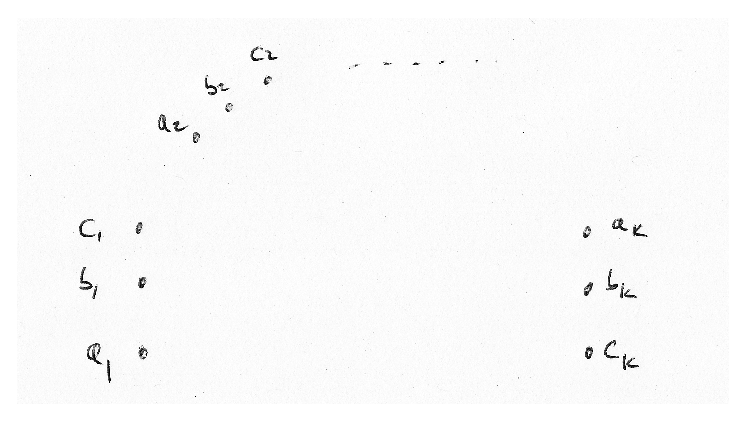
\includegraphics[height=30mm]{images/3sat-graph.eps}
\end{center}
}
\es

\bs{$CLIQUE$}
{\small
We construct the edges by connecting all the nodes except for
\begin{itemize}
\item nodes that are in the same triple, and
\item nodes that have contradictory labels, i.e., $x$ and $\ol{x}$.
\end{itemize}

Example construction using 
\[
\phi_3=(x_1 \vee x_1 \vee x_2) \wedge
	(\ol{x_1} \vee \ol{x_2} \vee \ol{x_2}) \wedge
	(\ol{x_1} \vee x_2 \vee x_2)
\]
gives rise to the graph
\begin{center}
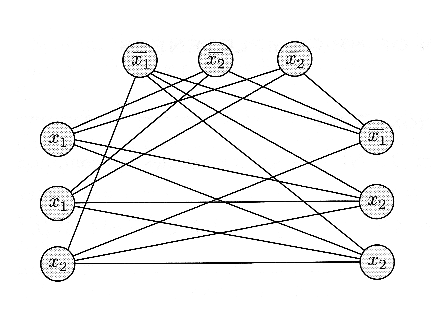
\includegraphics[height=25mm]{images/3sat-graph-2.eps}
\end{center}
}
\es


\bs{$CLIQUE$}
{\small
It is easy to see that this is a polynomial time construction (let $n$ be the number of
nodes then we see that algorithm runs in $O(n^2)$ time).

We now have to verify the reduction condition
\[
\phi_k \in 3SAT \mbox{ iff } f(\phi_k) \in CLIQUE
\]
First the '$\Rightarrow$' direction, suppose that $\phi_k$ has a satisfying assignment,
that means that each clause has at least one literal that is true.
In each triple of $G$ we choose one node that corresponds to a true literal.
The number of nodes selected is $k$, one in each triple.
All the selected nodes are connected by edges.  This shows that a satisfying
assignment of $\phi_k$ produces a $k$-clique.

For the converse, assume that $G$ has a $k$-clique.  By construction, no two nodes
can occur in the same triple.  Therefore, each of the $k$ triple contain exactly
one of the $k$ clique nodes.  Each node in the $k$-clique denotes an assignment
to true for a literal in $\phi_k$.  This is always true because opposing literals are not
connected. $\Box$
}
\es

\bs{$HAMPATH$}
{\small
Recall that $HAMPATH = \{ \encode{G,s,t}|\mbox{$G$ is a directed graph with a Hamiltonian path from $s$ to $t$}\}$ and a Hamiltonian path is a path in a graph that goes through each node exactly once.

\ftheorem{
\[
HAMPATH \in \mbox{$NP$-complete}.
\]
}
{\bf Proof Sketch:} We know that $HAMPATH \in NP$.  It remains to show that
$A \le_p HAMPATH$, for all $A \in NP$.  We show this by a polynomial time reduction $f$
from $3SAT$ to $HAMPATH$,
\[
\phi_k \in 3SAT \mbox{ iff } f(\phi_k) \in HAMPATH,
\]
where $f(\phi_k) = \encode{G,s,t}$.

For details of the construction see the book$\ldots$
}
\es

\bs{$NP$-Hard}

\fdef{A language $Q$ is {\bf\em NP-hard} if it satisfies two conditions:
\begin{enumerate}
\item $Q \not\in NP$, and
\item every $Q_i \in NP$ is polynomial time reducible to $Q$.
\end{enumerate}}

\es

\bs{Traveling Salesman}
{\small
The idea is, given a set of cities (nodes) that are connected via roads (weighted edges), find the cheapest route through all the cities (find a Hamiltonian path that minimizes the sum of the weights
in the path).  Formally,

$TSP = \{ \encode{G,s,t,w} | G$ is directed weighted graph with a {\em minimal} Hamiltonian path of
weight $w$ from $s$ to $t \}.$
}
\es


\bs{Traveling Salesman}
{\small
\ftheorem{
\[
TSP \in \mbox{$NP$-hard}.
\]
}
{\bf Proof:}  Note, a problem is $NP$-hard if every $L \in NP$ can be reduced to it in polynomial time but the problem itself is not in $NP$.  No known $NP$ solution exists for $TSP$ ($NP$ problems have polynomial time verifiers; in $TSP$ it is not possible to verify a certificate in polynomial time).  It remains to show that all $L \in NP$ reduce to it in polynomial time.  We will show this by a polynomial time reduction  $f$ from $HAMPATH$  to $TSP$,
\[
\encode{G,s,t} \in HAMPATH \mbox{ iff } f(\encode{G,s,t}) \in TSP,
\]
where $f(\encode{G,s,t}) = \encode{G',s,t,m}$ with $G'$ the graph $G$ with a weight of $1$ on all of its edges
and $m$  the number of nodes in $G$.  Clearly, the reduction runs in polynomial time.  We verify the reduction condition by first observing that a Hamiltonian path gives rise to a minimal traveling salesman circuit by the virtue that all Hamiltonian paths in $G'$ have the same cost.  The converse also holds, if we have a traveling salesman circuit this implies that we have a Hamiltonian path. $\Box$
}
\es

\end{document}
%%%%%%%%%%%%%%%%%%%%%%%%%%% end of template1.tex %%%%%%%%%%%%%%%%%%%%%%%%%%%%%%%%

